\newpage
\section{モデル生物の構造およびロボット外殻の設計}
本研究ではモデル生物としてズワイガニを採用した.本章では先行研究\cite{hasegawa}にて行われた解剖にて得られた各部の寸法,
関節可動域,および関節構造に関する知見について述べる.
さらにカニの羽状筋および関節構造を数理モデルとして表現し,実際のズワイガニの可動域を再現できるようなロボットの設計について検討する.
%%%%%%%%%%%%%%%%%%%%%%%%%%%%%%%%%%%%%%%%%%%%%%%%%%%%%%%%%
\subsection{解剖によって得られた知見について}
\subsubsection{モデル生物(ズワイガニ)について}
本研究では外骨格を有するモデル生物として甲殻類の十脚目短尾下目ケセンガニ科のズワイガニを用いた.
理由として蟹の中でも入手しやすく,モデルサイズも大きく解剖時に内部構造等の確認や測定が比較的容易なためである.
図\ref{fig:zuwai}に先行研究にて解剖に用いたズワイガニを示す.解剖に用いたズワイガニは食用に冷凍されたものであり,解剖によって得られた可動域などが,
カニが能動的に動く際のものとは異なる可能性があるが,今回は考慮しないものとする.
%%%%%%%%%%%%%%%%%%%%%%%%%%%%%%%%%%%%%%%%%%%%%%%%%%%%%%%%%
\begin{figure}[b]
  \begin{minipage}[b]{0.49\hsize}
    \centering
    \includegraphics[scale=0.05]{image/apearance3_1.png}
    \caption{解剖に用いたズワイガニ\cite{hasegawa}}
    \label{fig:zuwai}
  \end{minipage}
  %
  \begin{minipage}[b]{0.49\hsize}
    \vspace{10mm}
    \centering
    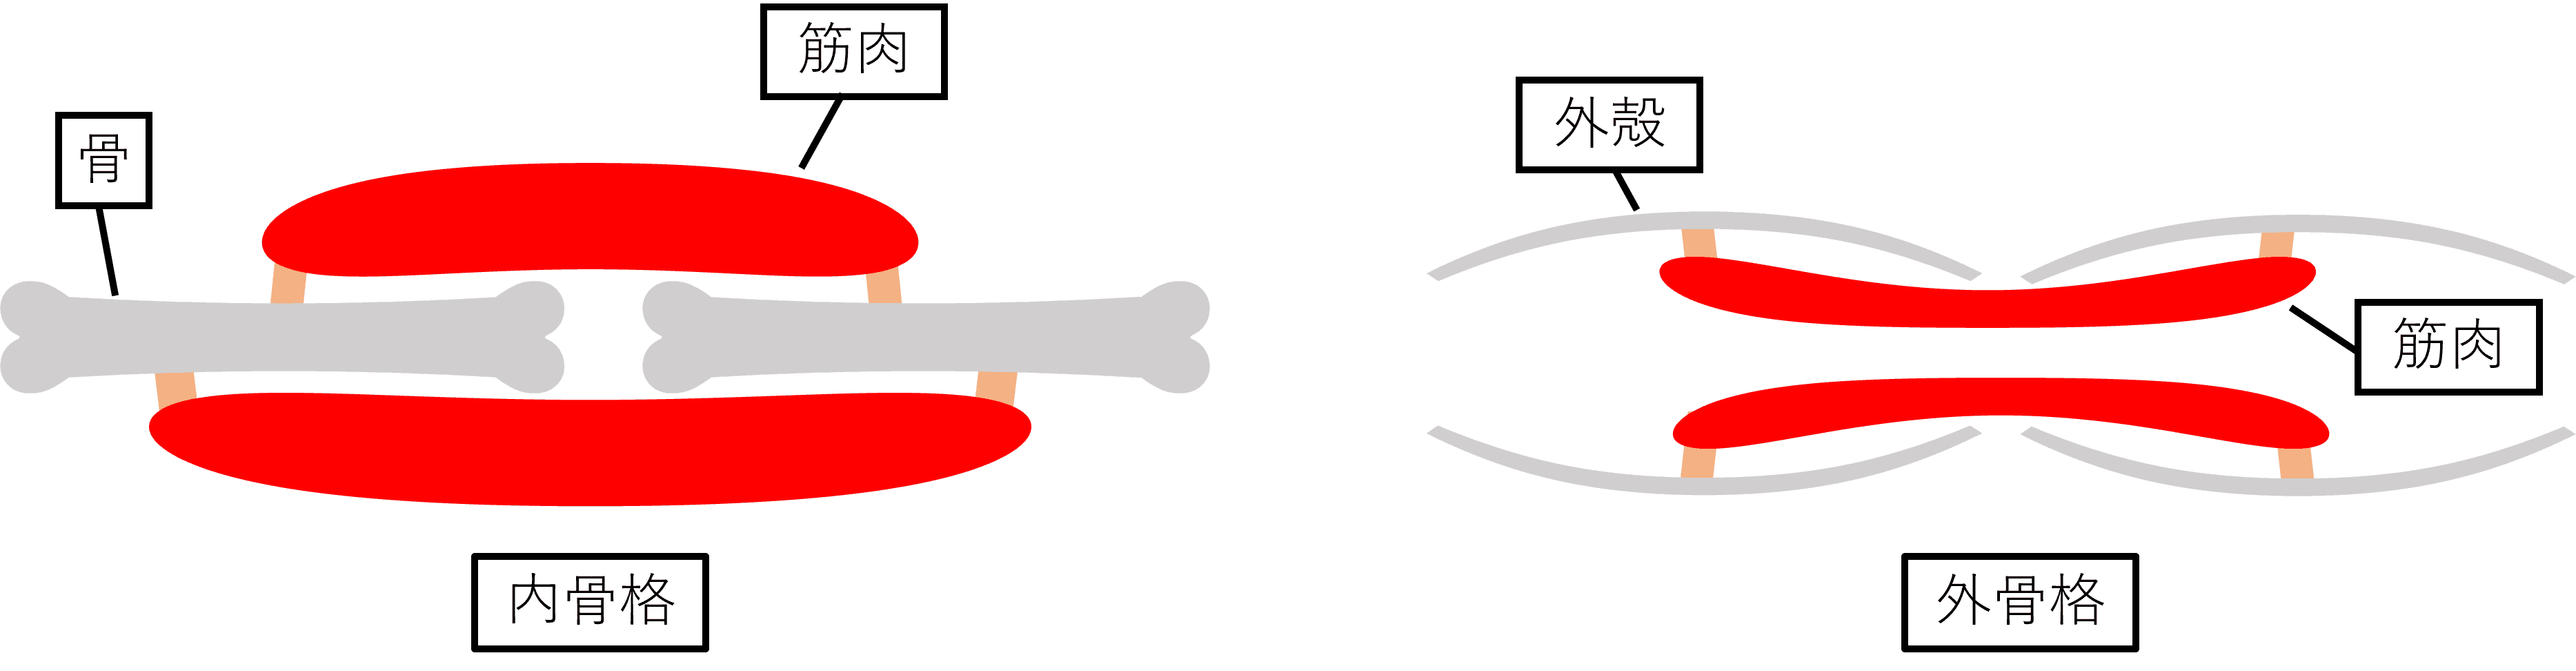
\includegraphics[scale=0.058]{image/kokkaku.png}
    \vspace{5mm}
    \caption{内骨格と外骨格\cite{hasegawa}}
    \label{fig:naigai}
  \end{minipage}
\end{figure}
%%%%%%%%%%%%%%%%%%%%%%%%%%%%%%%%%%%%%%%%%%%%%%%%%%%%%%%%%
\subsubsection{外骨格および羽状筋について}
内骨格と外骨格の筋肉の付着の仕方を簡易的に示したものを図\ref{fig:naigai}に示す.
我々人間などの脊椎動物の骨のように身体の内部にあり筋肉の付着点となり,身体を支持する骨格を内骨格という.
それに対して本研究で扱う外骨格は身体を外側から覆い,体を支持し,内部を保護しつつ,筋肉の付着点となる硬い構造のことで甲殻類の外殻などが当てはまる.
外骨格は外敵からの防御にも重要な役割を果たしている反面,硬くて重い外骨格は身体の屈曲性や可動性を阻害することが多いが,甲殻類,昆虫類などは外骨格に多数の関節を持つため運動性に優れている.
しかし身体は完全に外骨格で覆われており成長が妨げられるため定期的に脱皮を行うことで身体を大きくしている.

蟹の脚内の筋肉の構造および関節駆動機構について述べる.蟹の脚内部を充填する筋繊維の一端は節の内壁に付着し,もう一方は腱と呼ばれる組織,いわゆる蟹のすじに付着する.
腱は隣の関節の端に繋がっており,筋繊維が収縮することによって腱が引っ張られ節が開閉する.
筋繊維は腱に対して斜めに充填されており,このように配置された筋繊維を羽状筋という.
羽状筋の動きの模式図を図\ref{fig:ujo}に示す.
図\ref{fig:ujo}の左側が筋肉が伸展した状態,右側が収縮した状態を表している.ここで筋肉と腱のなす角を羽状角という.筋肉が収縮することで羽状筋の角度は27 degから41 degに増加し,腱は距離dを移動する.
ここで各筋繊維は収縮することで短く太くなるが,筋全体の幅wは変化しない.
このような羽状筋の動作には2つの利点があるとされている.1つ目は収縮しても膨張せず,羽状筋の角度が大きくなるだけなので限られた狭い空間で働くのに適していること,
2つ目は同じ形状と体積の平行筋と比べ収縮時に約2倍の力を発揮することが出来ることである\cite{warner1977biology}.
%%%%%%%%%%%%%%%%%%%%%%%%%%%%%%%%%%%%%%%%%%%%%%%%%%%%%%%%%

\begin{figure}[t]
  \begin{minipage}[b]{0.6\hsize}
    \centering
    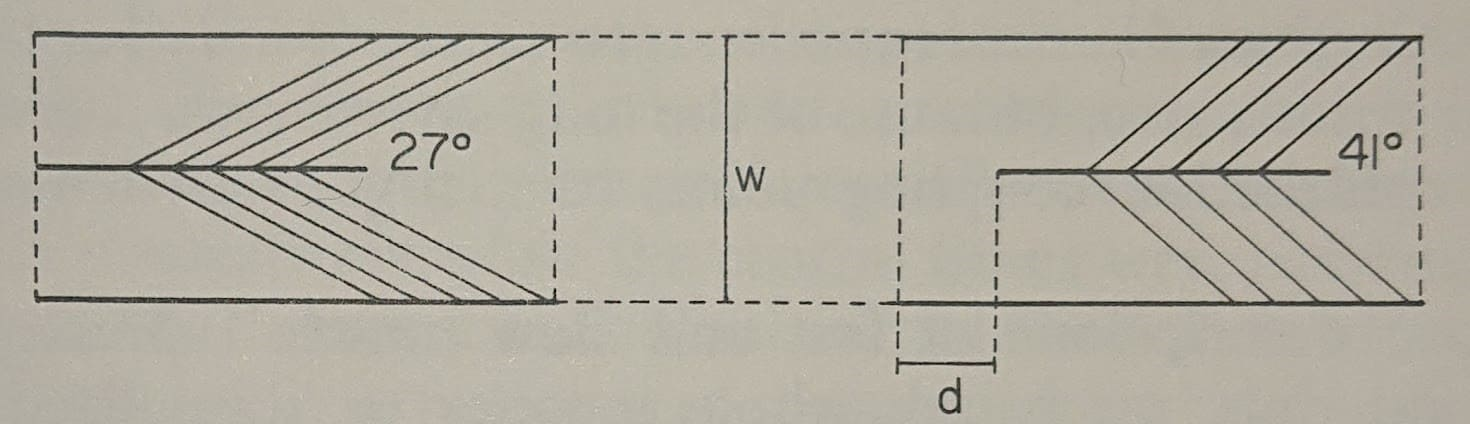
\includegraphics[scale=0.18]{image/ujo.JPG}
    \vspace{5mm}
    \caption{羽状筋の動きを模式的に表したもの\cite{warner1977biology}}
    \label{fig:ujo}
  \end{minipage}
  %
  \begin{minipage}[b]{0.39\hsize}
    \centering
    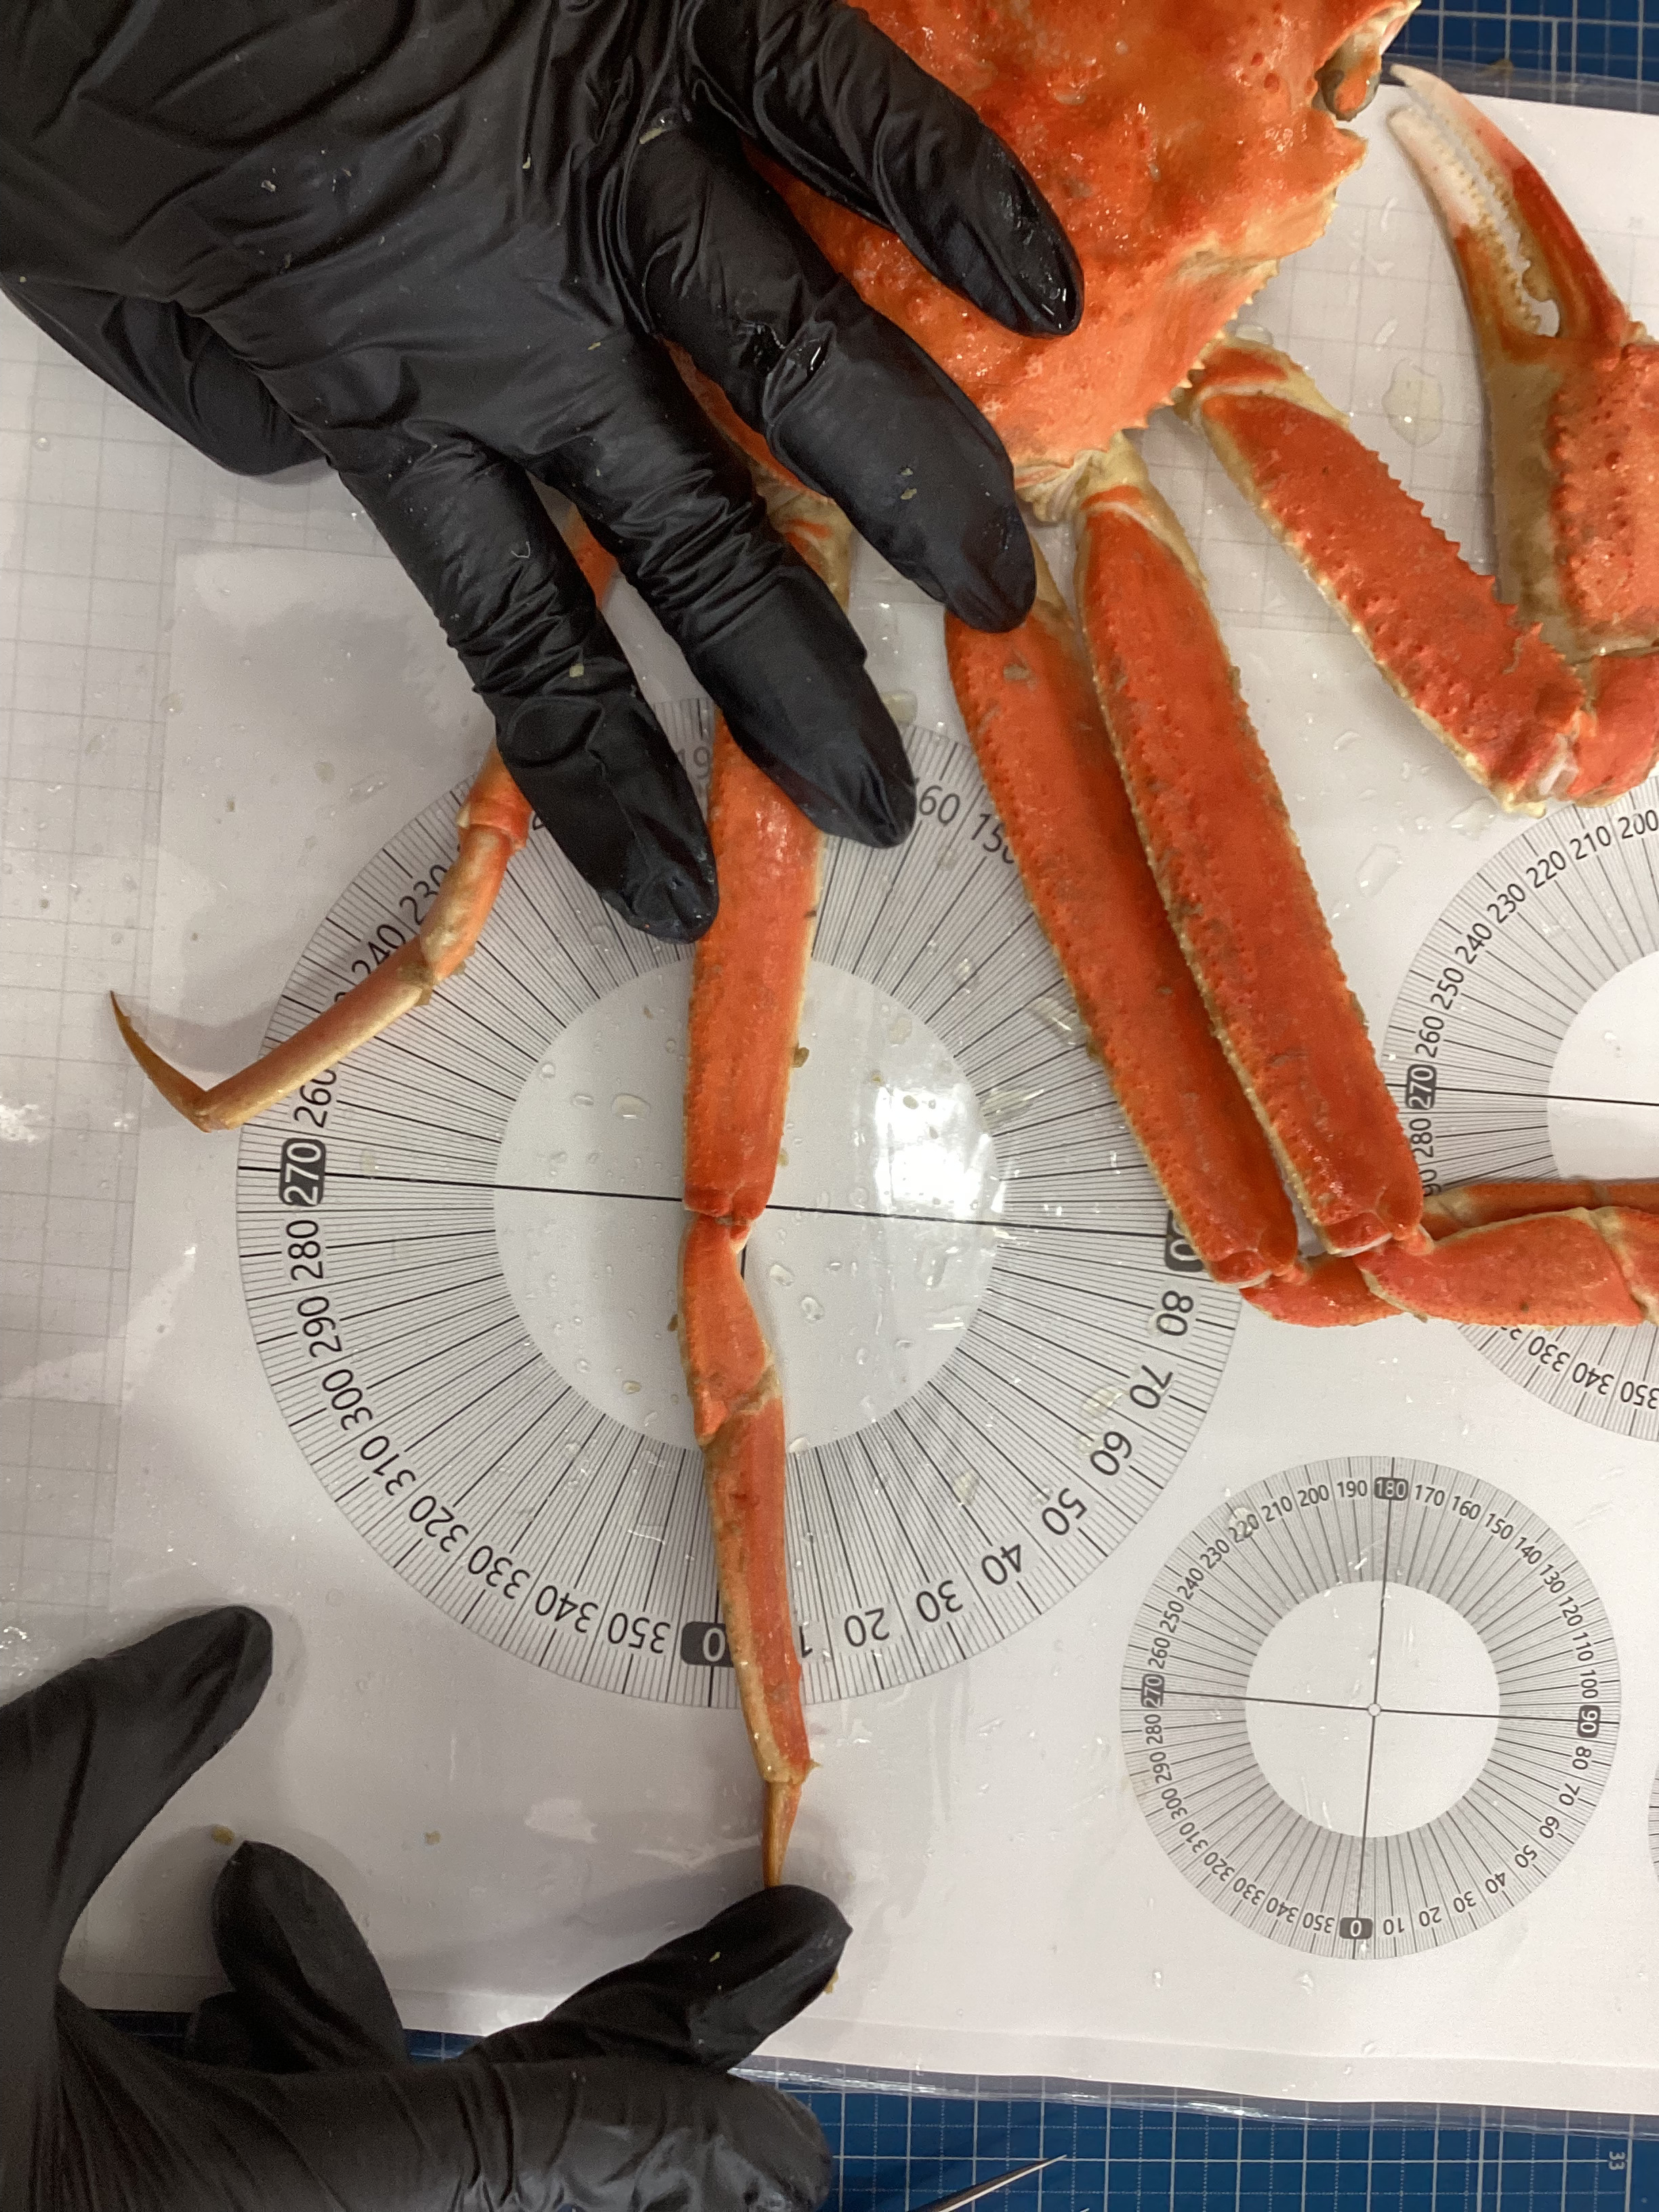
\includegraphics[scale=0.045]{image/degree_jikken.png}
    \caption{可動域の測定の様子}
    \label{fig:sokutei}
  \end{minipage}
\end{figure}
%%%%%%%%%%%%%%%%%%%%%%%%%%%%%%%%%%%%%%%%%%%%%%%%%%%%%%%%%
\begin{figure}[t]
  \centering
  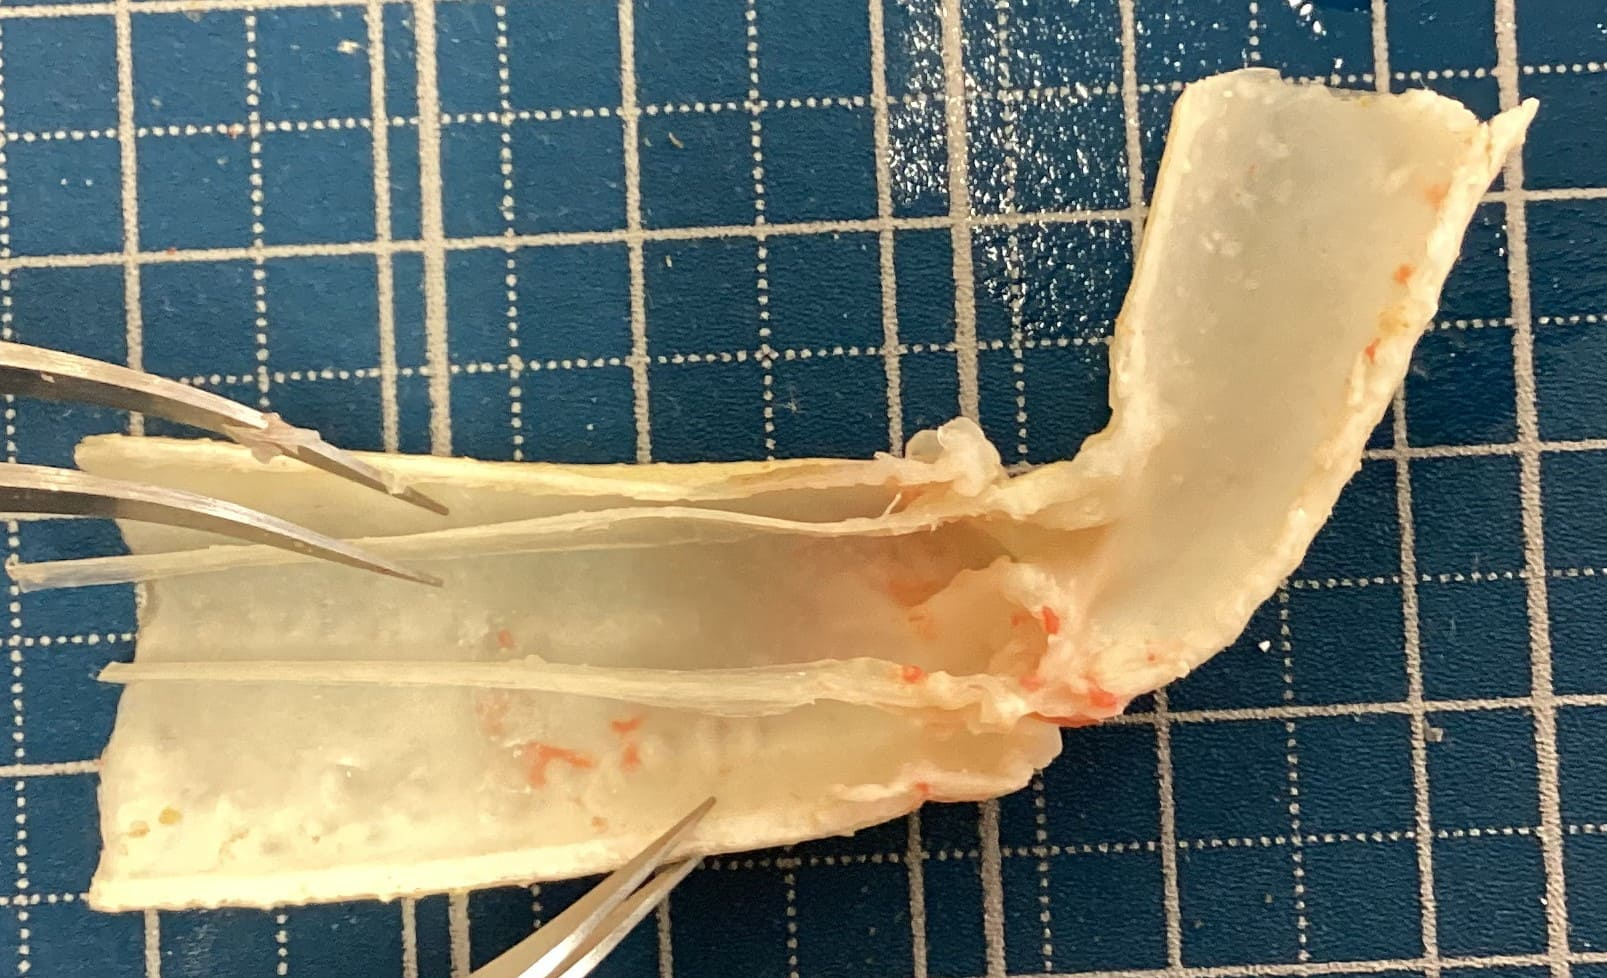
\includegraphics[scale=0.1]{image/setukanmaku.jpg}
  \caption{腱の様子\cite{hasegawa}}
  \label{fig:ken}
\end{figure}
%%%%%%%%%%%%%%%%%%%%%%%%%%%%%%%%%%%%%%%%%%%%%%%%%%%%%%%%%
\subsubsection{可動域,各部寸法,および可動域について}
先行研究\cite{hasegawa}にて行われた関節可動域の計測の様子を図\ref{fig:sokutei}に示す.
測定方法は,可動域を測定したい関節の軸を分度器の中心に合わせる.その時に関節の身体側の節の中心を 180°の線に合うように配置する.
そして蟹の脚で開閉動作を行い,脚先側の節の中心が閉じた状態と開いた状態での角度をそれぞれ測定してそれらを可動域とした.
なお,本研究では図\ref{fig:zuwai}中の4と書かれている下から4番目の節(第4肢)の可動域のデータを用いて機体を作製する.
第4肢の可動域を表\ref{tab:4setukadou}に示す.

また各節の長さについても測定が行われた.第4肢の長節から指節の寸法を表\ref{tab:4setu}に示す.
なお,実寸大では外骨格内部へアクチュエータの配置が困難なことから,後述する今回開発したロボットにおいては
長節,前節,指節では実測値に対して直径方向に7倍,直径方向には3.5倍,腕節は他の節より長手方向のみ5.2倍にした.
長手方向の具体的な寸法としては,長節が 350mm,腕節が 256mm,前節が 245mm,指節が 100mmである.
また先行研究\cite{hasegawa}でズワイガニを解剖した際に記録した長節-腕節間の腱の様子を図\ref{fig:ken}に示す.
解剖結果よりズワイガニの腱は節間膜と一体となっていることが分かった\cite{hasegawa}.
このような構造は関節内部への侵入を防ぐなど,外骨格として重要な役割をになっている可能性がある.
%%%%%%%%%%%%%%%%%%%%%%%%%%%%%%%%%%%%%%%%%%%%%%%%%%%%%%%%%
\begin{table}[t]
  \centering
  \vspace{5mm}
  \caption{第4肢の節間の可動域}
  \label{tab:4setukadou}
  \vspace{-3mm}
  \begin{tabular}{|l|c|}
  \hline
         & \multicolumn{1}{l|}{可動域 {[}deg{]}} \\ \hline
  長節-腕節間 & 52-130                            \\ \hline
  腕節-前節間 & 0-45                             \\ \hline
  前節-指節間 & 0-89                            \\ \hline
  \end{tabular}
\end{table}
%%%%%%%%%%%%%%%%%%%%%%%%%%%%%%%%%%%%%%%%%%%%%%%%%%%%%%%%% 
\begin{table}[t]
  \centering
  \caption{第4肢の長節から指節の寸法}
  \label{tab:4setu}
  \vspace{-3mm}
  \begin{tabular}{|l|c|c|c|c|c|}
  \hline
     & \multicolumn{1}{l|}{幅-左 [mm]} & \multicolumn{1}{l|}{幅-中 [mm]} & \multicolumn{1}{l|}{幅-右 [mm]} & \multicolumn{1}{l|}{厚み [mm]} & \multicolumn{1}{l|}{長さ [mm]} \\ \hline
  長節 & 19.10                       & 21.74                       & 13.11                       & 11.05                       & 100.0                       \\ \hline
  腕節 & 10.57                       & -                           & 18.42                       & 8.74                        & 40.5                        \\ \hline
  前節 & 16.48                       & -                           & 10.40                       & 4.68                        & 70.0                        \\ \hline
  指節 & -                           & 5.60                        & -                           & 3.69                        & 30.0                        \\ \hline
  \end{tabular}
\end{table}
%%%%%%%%%%%%%%%%%%%%%%%%%%%%%%%%%%%%%%%%%%%%%%%%%%%%%%%%%
\begin{figure}[t]
  %
  \begin{minipage}[b]{0.49\hsize}
    \centering  
    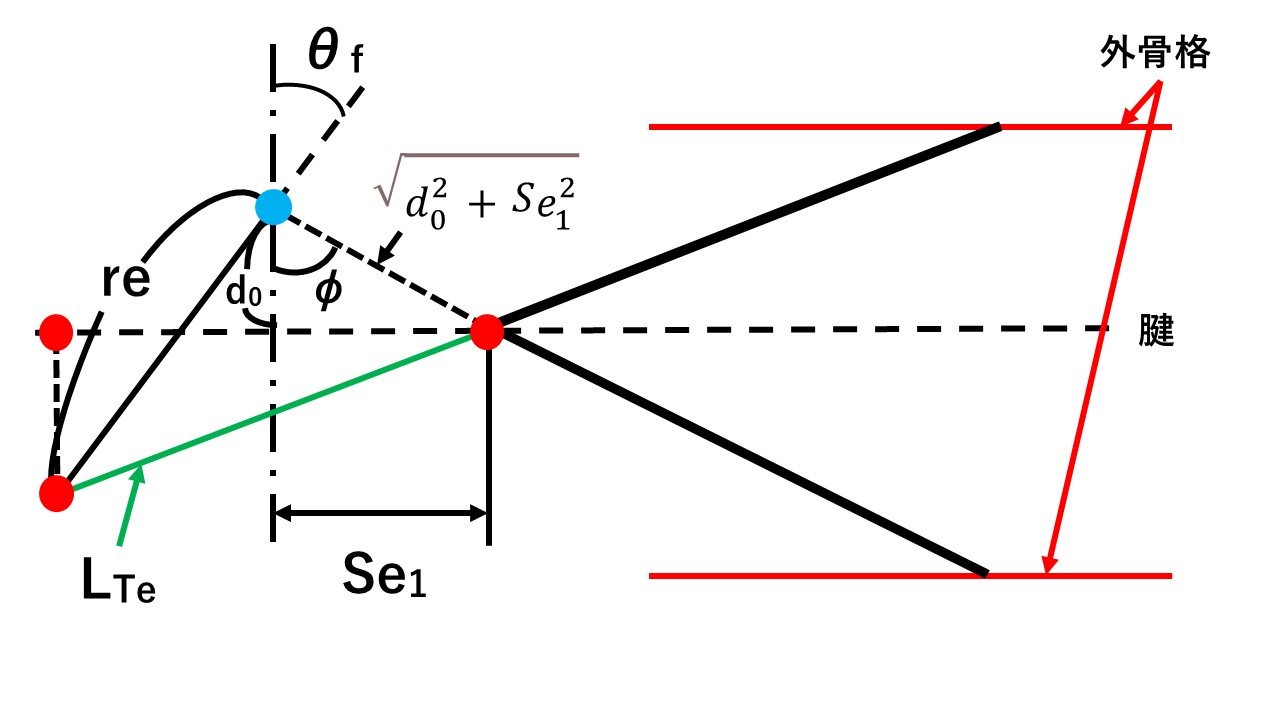
\includegraphics[scale=0.23]{image/model_1.jpg}
    \subcaption{圧縮空気印加前}
    \label{fig:model_1_before}
  \end{minipage}
  %
  \begin{minipage}[b]{0.49\hsize}
    \centering
    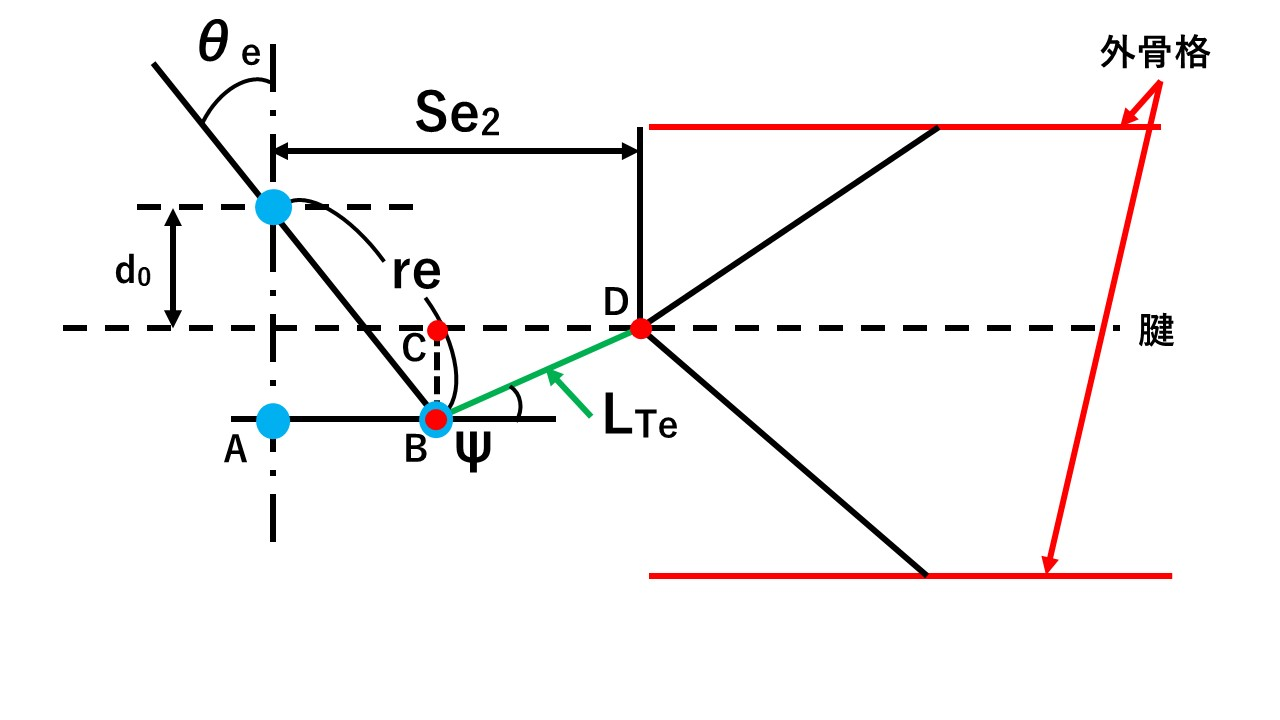
\includegraphics[scale=0.23]{image/model_2.jpg}
    \subcaption{圧縮空気印加後}
    \label{fig:model_1_after}
  \end{minipage}
  %
  \caption{可動域計算に用いた数理モデル(必要ストローク)}
  \label{fig:model_1}
\end{figure}
%%%%%%%%%%%%%%%%%%%%%%%%%%%%%%%%%%%%%%%%%%%%%%%%%%%%%%%%%
\subsection{羽状筋および関節構造のモデル化および可動域の計算}
\subsubsection{羽状筋および関節構造のモデル化}
作製する歩脚ロボットの可動域を設計するために,カニの関節構造を数理モデル化し,計算を行った.数理モデルを図\ref{fig:model_1}に示す.
モデルは伸筋による関節の開閉を表しており,図\ref{fig:model_1}\subref{fig:model_1_before}が関節が最も閉じて筋が引き延ばされた状態,
図\ref{fig:model_1}\subref{fig:model_1_after}が筋肉が収縮し関節が最も閉じている状態である.
図\ref{fig:model_1},\ref{fig:model_2}中に用いた変数について表\ref{tab:hensu}に示す.
%%%%%%%%%%%%%%%%%%%%%%%%%%%%%%%%%%%%%%%%%%%%%%%%%%%%%%%%%
可動域導出の手順について述べる.
まず図\ref{fig:model_1}\subref{fig:model_1_before}から,伸び縮みしない腱の長さ$L_{Te}$を求める.
腱付着点から腱の延長線に向かって垂線を引く.赤い点を頂点とする三角形において三平方の定理を用いて$L_{Te}$を求める.
\begin{equation}
  L_{Te} = \sqrt{r_e^2 + (d_0^2 + S_{e1}^2) - 2r_e\sqrt{d_0^2 + S_{e1}^2}\cos (\theta_f + \phi ) } 
\end{equation}
続いて図\ref{fig:model_1}\subref{fig:model_1_after}から,$S_{e2}$を求める.
青い点を頂点とする三角形の辺ABと赤い点を頂点とする三角形の辺CDを足し合わせて$S_{e2}$を求める.
\begin{equation}
  S_{e2} = r_e\sin \theta_e + L_{Te}\cos \psi  
\end{equation}
\begin{equation}
  \psi  = \sin^{-1}({\dfrac{r_e \cos \theta_e - d_0}{L_{Te}}})
\end{equation}
ここで,可動域$\theta_e + \theta_f$を実現するためには,腱は$S_{e2} - S_{e1}$の長さを移動しなければならない.
そこでこの移動距離を必要ストローク$S_e = S_{e2} - S_{e1}$と定義する.

一方で,実際のロボットにおいては初期羽状角と空圧筋の収縮率がわかっていれば,収縮によって腱がどれ程引き込まれるかは計算することができる.
この実際の腱の移動量を可能ストローク$S_{e}^{'}$と定義する.
本研究において設計した外骨格内部に配置された羽状筋が取り得る最小羽状角である 20度を,初期羽状角として設定した.また後述(4.3)するように,本研究で用いる改良型の細径MPAは最大収縮率が 20%である.
以上の条件および図\ref{fig:model_2}から,腱がどれ程引き込まれるか計算した.
圧縮空気印加前の細径MPAの長さが$l_1$とすると印加後の長さは収縮率が 20%なので$l_2 = 0.8l_1$となる.
このことを用いて$ S_{e}^{'}$を求める.
\begin{equation}
  \begin {split}
  S_{e}^{'}  & = l_1\cos\theta_1 + l_2\cos\theta_2\\
       & = l_1\cos20° + 0.8l_1\cos\theta_2
  \end{split}
\end{equation}
\begin{equation}
  \theta_2 = \sin^{-1}({\dfrac{d}{0.8 l_1}})
\end{equation}
表\ref{tab:parameta_1_1}~\ref{tab:parameta_3_2}に長節から指節までの各関節のパラメータを示す.
%%%%%%%%%%%%%%%%%%%%%%%%%%%%%%%%%%%%%%%%%%%%%%%%%%%%%%%%%
\begin{table}[htbp]
  \centering
  \vspace{5mm}
  \caption{可動域の計算に用いた変数}
  \label{tab:hensu}
  \vspace{-3mm}
  \scalebox{0.8}{
  \begin{tabular}{|l|c|}
  \hline
  $\theta_f[\textrm {deg}] $ & 関節から腱への垂線と,腱の付着点から関節への直線とのなす角                            \\ \hline
  $ \phi[\textrm {deg}]    $ & 
  \begin{tabular}{c}
  関節から腱への垂線と,関節から\\関節側にある細径MPAの交点への直線とのなす角
  \end{tabular}\\ \hline
  $  r_e[\textrm {mm}]     $ & 関節から腱の付着点までの長さ                                                       \\ \hline
  $ d_0[\textrm {mm}]     $ & 関節から腱への垂線の長さ                                                           \\ \hline
  $ L_{Te}[\textrm {mm}]    $ & 腱付着点から関節側にある細径MPAの交点までの長さ                                      \\ \hline
  $ S_{e1}[\textrm {mm}]    $ & 
  \begin{tabular}{c}
  関節から腱への垂線と腱との交点から\\関節側にある細径MPAの交点までの長さ
  \end{tabular}\\ \hline
  $\theta_e[\textrm {deg}] $ & 関節から腱への垂線と,腱の付着点から関節への直線とのなす角                            \\ \hline
  $ \psi[\textrm {deg}]    $ & 関節側の細径MPAの交点から腱の付着点の直線と水平な直線とのなす角                        \\ \hline
  $ S_{e2}[\textrm {mm}]    $ & 
  \begin{tabular}{c}
  関節から腱への垂線と腱との交点から\\関節側にある細径MPAの交点までの長さ
  \end{tabular}\\ \hline
  $ l_1[\textrm {mm}]     $ & 細径MPA動作前の細径MPAの長さ                                                       \\ \hline
  $\theta_1[\textrm {deg}] $ & 細径MPA動作前の羽状角の大きさ                                                      \\ \hline
  $ l_2[\textrm {mm}]     $ & 細径MPA動作後の細径MPAの長さ                                                       \\ \hline
  $\theta_2[\textrm {deg}] $ & 細径MPA動作後の羽状角の大きさ                                                      \\ \hline
  $d[\textrm {mm}]        $ & 腱から外骨格までの垂直距離                                                         \\ \hline
  \end{tabular}
  }
\end{table}
%%%%%%%%%%%%%%%%%%%%%%%%%%%%%%%%%%%%%%%%%%%%%%%%%%%%%%%%%
%
\begin{figure}[htbp]
  %
  \begin{minipage}{0.49\hsize}
    \centering  
    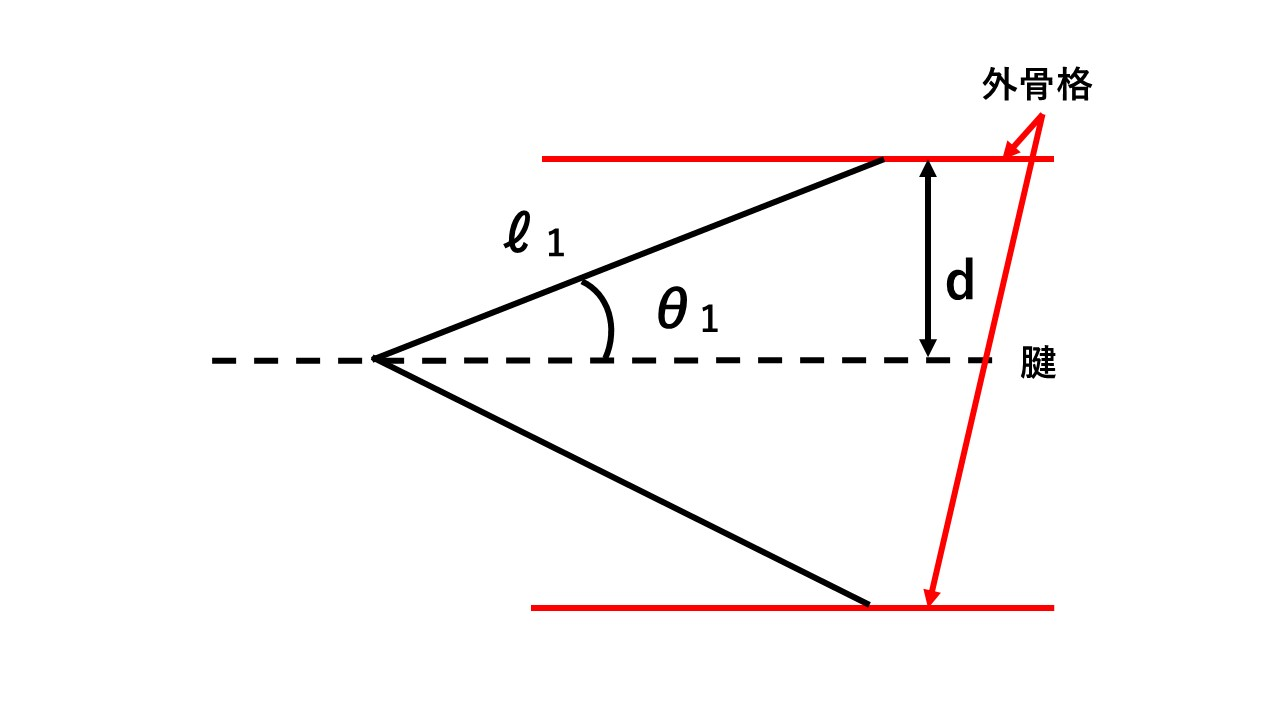
\includegraphics[scale=0.23]{image/model_2_open.jpg}
    \subcaption{圧縮空気印加前}
    \label{fig:model_2_before}
  \end{minipage}
  %
  \begin{minipage}{0.49\hsize}
    \centering
    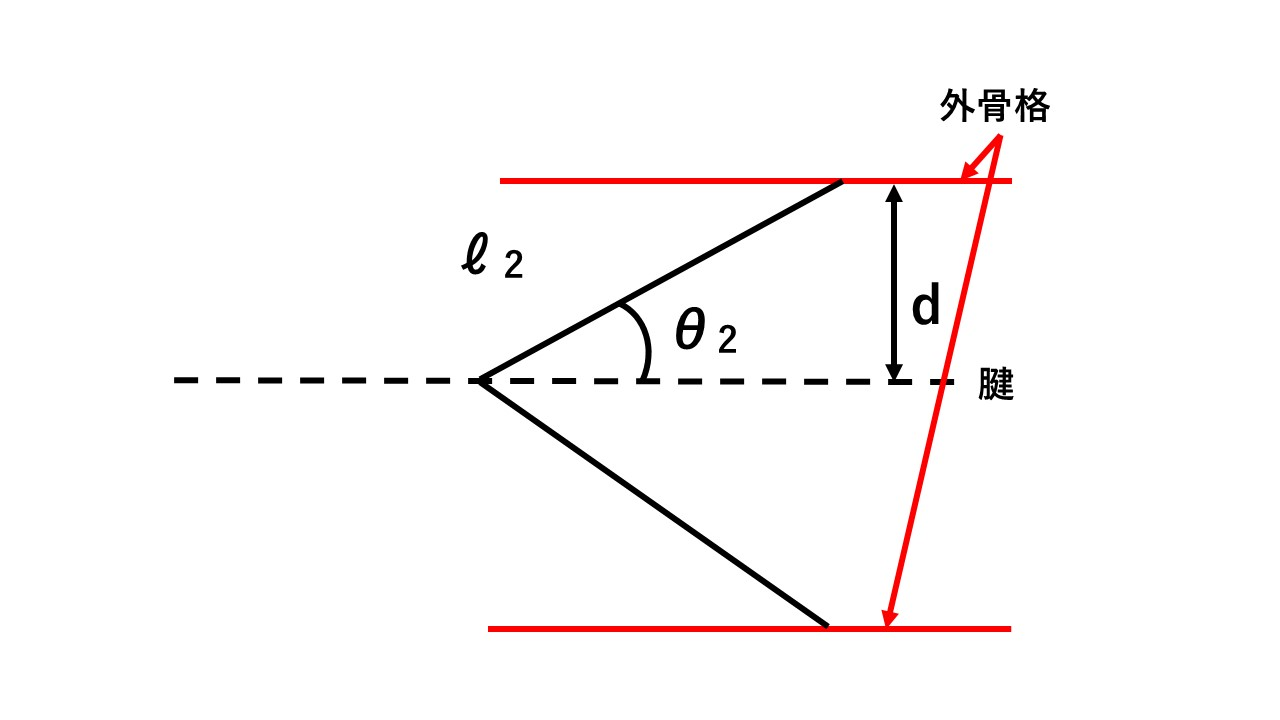
\includegraphics[scale=0.23]{image/model_2_close.jpg}
    \subcaption{圧縮空気印加後}
    \label{fig:model_2_after}
  \end{minipage}
  %
  \caption{可動域計算に用いた数理モデル(可能ストローク)}
  \label{fig:model_2}
\end{figure}
%%%%%%%%%%%%%%%%%%%%%%%%%%%%%%%%%%%%%%%%%%%%%%%%%%%%%%%%%
\begin{table}[htbp]
  \begin{minipage}{1\hsize}
    \centering
    \vspace{-7mm}
    \caption{長節-腕節間(開筋)のパラメータ}
    \label{tab:parameta_1_1}
    \vspace{-3mm}
    \scalebox{0.8}{
    \begin{tabular}{|c|c|c|c|c|c|c|c|c|c|c|c|c|c|c|c|}
    \hline
    $\theta _f [\textrm{deg}]$ & $\phi [\textrm{deg}]$ & $r_e [\textrm{mm}]$ &  $d_0 [\textrm{mm}]$ & $L_{Te} [\textrm{mm}]$ & $S_{e1} [\textrm{mm}]$ & $\theta_e [\textrm{deg}]$ & $\psi [\textrm{deg}]$ \\ \hline
    39.5 & 64.3 & 24.7 & 17.0 & 51.1 & 35.3 & 51.5 & 11.5  \\ \hline
    $S_{e2} [\textrm{mm}]$ & $l_1 [\textrm{mm}]$ & $\theta_1 [\textrm{deg}]$ & $l_2 [\textrm{mm}]$ & $\theta_2 [\textrm{deg}]$ & $d [\textrm{mm}]$ & $S_e [\textrm{mm}]$ & $S_{e}^{'} [\textrm{mm}]$ \\ \hline
    69.4 & 156 & 20.0 & 125 & 25.3 & 53.4 & 34.1 & 31.0 \\ \hline
    \end{tabular}
    }
  \end{minipage}
  %
  \begin{minipage}{1\hsize}
    \centering
    \caption{長節-腕節間(閉筋)のパラメータ}
    \label{tab:parameta_1_2}
    \vspace{-3mm}
    \scalebox{0.8}{
    \begin{tabular}{|c|c|c|c|c|c|c|c|}
    \hline
    $\theta _f [\textrm{deg}]$ & $\phi [\textrm{deg}]$ & $r_e [\textrm{mm}]$ &  $d_0 [\textrm{mm}]$ & $L_{Te} [\textrm{mm}]$ & $S_{e1} [\textrm{mm}]$ & $\theta_e [\textrm{deg}]$ & $\psi [\textrm{deg}]$ \\ \hline
    39.5 & 64.3  & 24.9 & 17.0 & 64.2 & 35.3 & 51.5 & 11.5  \\ \hline
    $S_{e2} [\textrm{mm}]$ & $l_1 [\textrm{mm}]$ & $\theta_1 [\textrm{deg}]$ & $l_2 [\textrm{mm}]$ & $\theta_2 [\textrm{deg}]$ & $d [\textrm{mm}]$ & $S_e [\textrm{mm}]$ & $S_{e}^{'} [\textrm{mm}]$ \\ \hline
    \end{tabular}
    }
  \end{minipage}
\end{table}
 %
\begin{table}[htbp]
  \begin{minipage}{1\hsize}
    \centering
    \vspace{-15mm}
    \caption{腕節-前節間(開筋)のパラメータ}
    \label{tab:parameta_2_1}
    \vspace{-3mm}
    \scalebox{0.8}{
    \begin{tabular}{|c|c|c|c|c|c|c|c|}
      \hline
      $\theta _f [\textrm{deg}]$ & $\phi [\textrm{deg}]$ & $r_e [\textrm{mm}]$ &  $d_0 [\textrm{mm}]$ & $L_{Te} [\textrm{mm}]$ & $S_{e1} [\textrm{mm}]$ & $\theta_e [\textrm{deg}]$ & $\psi [\textrm{deg}]$ \\ \hline
      45 & 90.0  & 27.1 & 0 & 44.9 & 19.0 & 0 & 0.707  \\ \hline
      $S_{e2} [\textrm{mm}]$ & $l_1 [\textrm{mm}]$ & $\theta_1 [\textrm{deg}]$ & $l_2 [\textrm{mm}]$ & $\theta_2 [\textrm{deg}]$ & $d [\textrm{mm}]$ & $S_e [\textrm{mm}]$ & $S_{e}^{'} [\textrm{mm}]$ \\ \hline
      14.6 & 57.8 & 20.0 & 46.2 & 25.3 & 19.8 & 13.6 & 11.6 \\ \hline
      \end{tabular}
      }
    \end{minipage}
  %
  \begin{minipage}{1\hsize}
    \centering
    \vspace{2mm}
    \caption{腕節-前節間(閉筋)のパラメータ}
    \label{tab:parameta_2_2}
    \vspace{-3mm}
    \scalebox{0.8}{
      \begin{tabular}{|c|c|c|c|c|c|c|c|}
        \hline
        $\theta _f [\textrm{deg}]$ & $\phi [\textrm{deg}]$ & $r_e [\textrm{mm}]$ &  $d_0 [\textrm{mm}]$ & $L_{Te} [\textrm{mm}]$ & $S_{e1} [\textrm{mm}]$ & $\theta_e [\textrm{deg}]$ & $\psi [\textrm{deg}]$ \\ \hline
        68.7 & 90.0  & 24.9 & 0 & 49.7 & 18.8 & 21.6 & 33.7  \\ \hline
        $S_{e2} [\textrm{mm}]$ & $l_1 [\textrm{mm}]$ & $\theta_1 [\textrm{deg}]$ & $l_2 [\textrm{mm}]$ & $\theta_2 [\textrm{deg}]$ & $d [\textrm{mm}]$ & $S_e [\textrm{mm}]$ & $S_{e}^{'} [\textrm{mm}]$ \\ \hline
        30.3 & 57.8 & 20.0 & 46.2 & 25.3 & 19.8 & 25.5 & 11.6 \\ \hline
        \end{tabular}
        }
      \end{minipage}
\end{table}
%
\begin{table}[htbp]
\begin{minipage}{1\hsize}
  \vspace{-15mm}
  \centering
  \caption{前節-指節間(開筋)のパラメータ}
  \label{tab:parameta_3_1}
  \vspace{-3mm}
  \scalebox{0.8}{
    \begin{tabular}{|c|c|c|c|c|c|c|c|}
      \hline
      $\theta _f [\textrm{deg}]$ & $\phi [\textrm{deg}]$ & $r_e [\textrm{mm}]$ &  $d_0 [\textrm{mm}]$ & $L_{Te} [\textrm{mm}]$ & $S_{e1} [\textrm{mm}]$ & $\theta_e [\textrm{deg}]$ & $\psi [\textrm{deg}]$ \\ \hline
      80 & 90.0  & 16.7 & 0 & 78.9 & 78.9 & 0 & 12.6  \\ \hline
      $S_{e2} [\textrm{mm}]$ & $l_1 [\textrm{mm}]$ & $\theta_1 [\textrm{deg}]$ & $l_2 [\textrm{mm}]$ & $\theta_2 [\textrm{deg}]$ & $d [\textrm{mm}]$ & $S_e [\textrm{mm}]$ & $S_{e}^{'} [\textrm{mm}]$ \\ \hline
      90.5 & 58.5 & 20.0 & 46.8 & 25.3 & 20.0 & 9.81 & 11.7 \\ \hline
      \end{tabular}
      }
  \end{minipage}
\end{table}
%
\begin{table}[htbp]
\begin{minipage}{1\hsize}
  \centering
  \vspace{-15mm}
  \caption{前節-指節間(閉筋)のパラメータ}
  \label{tab:parameta_3_2}
  \vspace{-3mm}
  \scalebox{0.8}{
    \begin{tabular}{|c|c|c|c|c|c|c|c|}
      \hline
      $\theta _f [\textrm{deg}]$ & $\phi [\textrm{deg}]$ & $r_e [\textrm{mm}]$ &  $d_0 [\textrm{mm}]$ & $L_{Te} [\textrm{mm}]$ & $S_{e1} [\textrm{mm}]$ & $\theta_e [\textrm{deg}]$ & $\psi [\textrm{deg}]$ \\ \hline
      88.0 & 90.0  & 16.7 & 0 & 78.9 & 78.9 &1.00 & 27.2  \\ \hline
      $S_{e2} [\textrm{mm}]$ & $l_1 [\textrm{mm}]$ & $\theta_1 [\textrm{deg}]$ & $l_2 [\textrm{mm}]$ & $\theta_2 [\textrm{deg}]$ & $d [\textrm{mm}]$ & $S_e [\textrm{mm}]$ & $S_{e}^{'} [\textrm{mm}]$ \\ \hline
      90.5 & 58.5 & 20.0 & 46.8 & 25.3 & 20.0 & 11.5 & 11.7 \\ \hline
      \end{tabular}
      }
\end{minipage}
\end{table}